\documentclass[10pt,a4paper]{article}
\usepackage[utf8x]{inputenc}
\usepackage{ucs}
\usepackage[left=2.00cm, right=2.00cm, top=2.00cm, bottom=2.00cm]{geometry}
\renewcommand\familydefault{\sfdefault}

\title{Summary - \lecture}
\author{}
\date{}


%costum layout
\setlength{\parindent}{0cm}
\usepackage{fancyhdr}
\pagestyle{fancy}
\fancyhf{}
\fancyhead[L]{
	\strut\rlap{\colorlayout\rule[-\dp\strutbox]{\headwidth}{\headheight}}
	\textcolor {white} {Summary: \lecture}}
\fancyfoot[L]{
	\strut\rlap{\colorlayout\rule[-\dp\strutbox]{\headwidth}{\headheight}}
	\textcolor {white} {last changed: \today}}
\fancyhead[R]{\textcolor{white}{\semseter}}
\fancyfoot[R]{\textcolor{white} {\thepage}}


%math
\usepackage{amsmath}
\usepackage{amsfonts}
\usepackage{amssymb}
\usepackage{amstext}
\usepackage{mathtools}


%graphics
\usepackage{graphicx}
\usepackage{floatflt}
\usepackage{float}


%tabular
\usepackage{tabularx}
\usepackage[font=small,labelfont=small]{caption}
\usepackage{colortbl}
\usepackage[dvipsnames]{xcolor}
\renewcommand{\arraystretch}{1.5}
%\arrayrulecolor{white}


%tikz
\usepackage{tikz}
\usetikzlibrary{shapes, petri}
\tikzstyle{ell}=[ellipse,draw, yshift=-2mm]
\tikzstyle{rec} = [rectangle, draw]
\tikzstyle{dia} = [diamond, aspect=2, draw, yshift=-5mm]
\tikzstyle{cir} = [circle, draw, minimum size=3mm]
\tikzstyle{arrHV} = [to path={-| (\tikztotarget)}]
\tikzstyle{arrVH} = [to path={|- (\tikztotarget)}]
\tikzstyle{whileright} = [xshift=20mm, yshift=-3mm]
\tikzstyle{whileleft} = [xshift=-20mm, yshift=-3mm]
\tikzstyle{txtright} = [above, xshift=15mm]
\tikzstyle{txtleft} = [above, xshift=-15mm]
\tikzstyle{empty} = [coordinate]
\usetikzlibrary{positioning}


%listings
\usepackage{listings}
\lstdefinestyle{costum} {
	language=Bash,
	basicstyle=\footnotesize\ttfamily,
	keywordstyle=\bfseries\color{cyan!50!blue},
	commentstyle=\itshape\color{black!50},
	%identifierstyle=\color{blue},
	stringstyle=\color{green!50!black},
	morekeywords={returns, loop, each},
	escapeinside={\%*}{*)}
}
\lstset{style=costum}


%%custom title color
%\usepackage{titlesec}
%\setcounter{secnumdepth}{4}
%
%\titleformat{\section}
%{\color{cyan!80!blue}\normalfont\Large\bfseries}
%{\color{black}\thesection}{1em}{}
%
%\titleformat{\subsubsection}
%{\color{blue!30!black!70}\normalfont\bfseries}
%{\color{black}\thesection}{1em}{}
%
%\titleformat{\paragraph}
%{\color{green!30!black!70}\normalfont\normalsize\bfseries}{\theparagraph}{1em}{}
%\titlespacing*{\paragraph}
%{0pt}{3.25ex plus 1ex minus .2ex}{1.5ex plus .2ex}


%tab
\newcommand{\tab}[1][1]{\hspace*{#1cm}}


%hyperref
\usepackage{hyperref}


%vector
\newcommand{\vect}[1]{\ensuremath{\begin{bmatrix}#1\end{bmatrix}}}

%TODO
%config
\newcommand{\lecture}{Cyber-Physical Systems} %title of the lecture
\newcommand{\lecturer}{Althoff M.} %lecturer of the lecture
\newcommand{\semseter}{summer semester 2020} %semester of this lecture, e.g., summer semester 2019
\newcommand{\colorlayout}{\color{red!50!black}} %color of the title bar, see colors

%colors, e.g,
%cyan!50!blue
%green!50!black
%orange!50!black

%user


%TODO
% a user defined todo list


%%Check
%Introduction (y)
%FSA (y)
%



\begin{document}
\tableofcontents
\pagebreak

\section{Introduction}
\subsection{Typical Sensors and Actuators}
\begin{itemize}
	\item Sensors
	\begin{itemize}
		\item acceleration sensor
		\item light sensor
		\item force sensor
		\item temperature sensor
		\item video camera
		\item pressure sensor
		\item angle sensor
		\item LIDAR
	\end{itemize}
	\item Actuators
	\begin{itemize}
		\item electric motor
		\item hydraulic/pneumatic cylinder
		\item magnetic valve
		\item relay
		\item heating
		\item piezo actuator
		\item pump
		\item laser
	\end{itemize}
\end{itemize}

\subsection{Model-Based Design}
\subsubsection{Process}
\begin{enumerate}
	\item Modeling
	\item Design
	\item Analysis
	\item Deployment
\end{enumerate}

\subsubsection{Advantages}
\begin{itemize}
	\item Improvement of the product quality
	\item Handling complexity
	\item Shorter development times
\end{itemize}

\subsubsection{Concept of Systems}
\begin{itemize}
	\item \textbf{System:} Is a set of interacting or independent components that is distinguished from its environment by a system boundary
	\item \textbf{System boundary:} Describes the exchange of a system with its environment via inputs and outputs
	\item \textbf{Subsystem:} System in a system
\end{itemize}

\subsection{Signal Types}
\subsubsection{Continuous Signals}
$$
	f : \mathbb{R}^+_0 → \mathbb{R}
$$

\subsubsection{Discrete-Time Signal}
$$
	f : \mathcal D → \mathbb{R}
$$ where $\mathcal D$ is a countable set, e.g. $\mathcal D = \{t_1, t_2, \dots \} \text{ or } \mathcal D = \mathbb{N}_0$

\subsubsection{Discrete-Value Signal}
$$
	f : \mathbb{R}^+_0 → \mathcal D
$$ where $\mathcal D$ is a countable set, e.g. $\mathcal D  = \{0, 1\}$

\subsubsection{Discrete-Time and Discrete-Value Signal}
$$
	f : \mathcal D → \tilde{\mathcal D}
$$ where $\mathcal D, \tilde{\mathcal D}$ are countable sets

\subsection{Systems}
\begin{tabularx}{\columnwidth}{l|X|X|X}
	& Discrete-State System & Continuous-State System & Hybrid System \\
	\hline
	\hline
	States/Inputs/Outputs & discrete & continuous & discrete and continuous \\
	Time variable & $t_k$ (discrete) & $t$ (continuous) & $t$ (continuous)\\
	Input variable &  $u(t_k) \in \tilde{\mathcal D}_1$ & $u(t) \in \mathbb R$ & $u(t) \in \tilde{\mathcal D}_1$ or $\mathbb R$ \\
	Output variable &  $y(t_k) \in \tilde{\mathcal D}_2$ & $y(t) \in \mathbb R$ & $y(t) \in \tilde{\mathcal D}_2$ or $\mathbb R$ \\
	State vector & $z(t_k)$ & $x(t)$ & $x(t)$ \\
	Equations & $z(t_{k+1}) = A z(t_k) + b u(t_k)$ & $\dot x(t) = A x(t) + b u(t)$ & $\dot x(t) = A x(t) + b u(t)$ \\
	& $y(t_k) = c^T z(t_k)$ & $y(t) = c^T x(t)$ & $y(t) = c^T x(t)$
	
\end{tabularx}

\subsubsection{Properties}


\textbf{State of a dynamic system}
\begin{itemize}
	\item A state vector $x$ consists of the (smallest) number of variables that need to be specified at the initial time $t_0$ so that the future behavior is uniquely defined for a given input signal $u(t)$
\end{itemize}

\textbf{Static and Dynamic Systems}
\begin{itemize}
	\item \textbf{Static System:} No state required
	\item \textbf{Dynamic System:} State required
\end{itemize}

\textbf{Time-Invariant and Time-Variant Systems}
\begin{itemize}
	\item \textbf{Time-invariant system:} Shift of time does not change the outcome
	\item \textbf{Time-variant system:} Shift of time alters the outcome
\end{itemize}

\textbf{Deterministic and Non-Deterministic Systems}
\begin{itemize}
	\item \textbf{Deterministic system:} For an initial state $x(0)$ and a given input signal $u(t)$, there exists a unique solution of the state and the output
	\item \textbf{Non-deterministic system:} The evolution of the state and the output is not uniquely determined by the initial state and the input signal
\end{itemize}

\textbf{Causal, Acausal, and anticausal Systems}
\begin{itemize}
	\item \textbf{Causal sytem:} The output only depends on past and current inputs
	\item \textbf{Acausal system:} The output also depends on future inputs
	\item \textbf{Anticausal system:} The output only depends on future inputs
\end{itemize}




\section{Finite State Automata (FSA)}
\subsection{Mealy Machine}
\subsubsection{Definition}
$$
	A_{mealy} = (\mathcal Z, \mathcal U, \mathcal Y, f, g, z(0))
$$ where
$$
	\begin{array}{ll}
	z(0) & \text{initial state} \\
	\mathcal Z = \{z_1, \dots, z_n\} & \text{set of states} \\
	\mathcal U = \{\tilde{u}_1, \dots, \tilde{u}_m\} & \text{set of input symbols (input alphabet)} \\
	\mathcal Y = \{\tilde y_1, \dots, \tilde y_o\} & \text{set of output symbols (output alphabet)}
	\end{array}
$$
$$
	\begin{array}{lll}
	f : \mathcal Z \times \mathcal U → \mathcal Z & \text{transition function} & z(k + 1) = f(z(k), u(k)) \\
	g : \mathcal Z \times \mathcal U → \mathcal Y & \text{output function} & y(k) = g(z(k), u(k)) \\
	\end{array}
$$

\subsubsection{Graphical Representation}
\begin{figure}[H]
	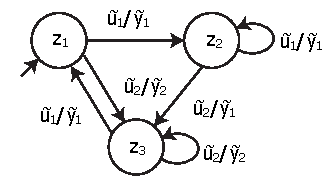
\includegraphics[width=0.7\columnwidth]{figures/fsm_mealy.pdf}
\end{figure}

\subsubsection{State Transition Table}
\begin{tabular}{cccc}
	\hline
	& \multicolumn{3}{c}{($z(k + 1), y(k)$) for $u(k)$} \\
	\hline
	$z(k)$ & $\tilde u_1$ & $\dots$ & $\tilde u_m$ \\
	\hline
	$z_1$ & ($z(k + 1), y(k)$) & $\dots$ & ($z(k + 1), y(k)$) \\
	$z_2$ & ($z(k + 1), y(k)$) & $\dots$ & ($z(k + 1), y(k)$) \\
	$\vdots$ & $\vdots$ & $\ddots$ & $\vdots$ \\
	\hline
\end{tabular}

\subsubsection{Transition Function and Output Function}
\textbf{Transition Function:} ~\\
$$
	f(z(k), u(k)) = \begin{cases}
		z_1 \text{ for} & ((z(k) = z_{i_1}) \land ((u(k) = \tilde u_{j_{11}}) \lor (u(k) = \tilde u_{j_{12}}) \lor \dots)) \lor \\
		& ((z(k) = z_{i_2}) \land ((u(k) = \tilde u_{j_{21}}) \lor (u(k) = \tilde u_{j_{22}}) \lor \dots)) \lor \\
		& \tab[3] \vdots \\
		z_2 \text{ for} & \dots \\
		\vdots & \tab[3] \vdots 
	\end{cases}
$$
where $z_{i_1}, z_{i_2}, \dots \in \mathcal Z$, $\tilde u_{j_{11}}, \tilde u_{j_{12}}, \dots, \tilde u_{j_{21}}, \dots \in \mathcal U$

\textbf{Output Function:} ~\\
$$
	g(z(k), u(k)) = \begin{cases}
		\tilde y_1 \text{ for} & ((z(k) = z_{i_1}) \land ((u(k) = \tilde u_{j_{11}}) \lor (u(k) = \tilde u_{j_{12}}) \lor \dots)) \lor \\
		& ((z(k) = z_{i_2}) \land ((u(k) = \tilde u_{j_{21}}) \lor (u(k) = \tilde u_{j_{22}}) \lor \dots)) \lor \\
		& \tab[3] \vdots \\
		\tilde y_2 \text{ for} & \dots \\
		\vdots & \tab[3] \vdots 
	\end{cases}
$$
where $z_{i_1}, z_{i_2}, \dots \in \mathcal Z$, $\tilde u_{j_{11}}, \tilde u_{j_{12}}, \dots, \tilde u_{j_{21}}, \dots \in \mathcal U$

\subsection{Moore Machine}
\subsubsection{Definition}
$$
	A_{moore} = (\mathcal Z, \mathcal U, \mathcal Y, f, g, z(0))
$$ where
$$
	\begin{array}{ll}
		z(0) & \text{initial state} \\
		\mathcal Z = \{z_1, \dots, z_n\} & \text{set of states} \\
		\mathcal U = \{\tilde{u}_1, \dots, \tilde{u}_m\} & \text{set of input symbols (input alphabet)} \\
		\mathcal Y = \{\tilde y_1, \dots, \tilde y_o\} & \text{set of output symbols (output alphabet)}
	\end{array}
$$
$$
	\begin{array}{lll}
		f : \mathcal Z \times \mathcal U → \mathcal Z & \text{transition function} & z(k + 1) = f(z(k), u(k)) \\
		g : \mathcal Z → \mathcal Y & \text{output function} & y(k) = g(z(k)) \\
	\end{array}
$$

\subsubsection{Graphical Representation}
\begin{figure}[H]
	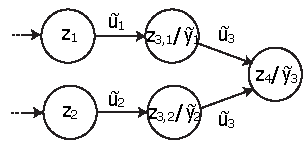
\includegraphics[width=0.7\columnwidth]{figures/fsm_moore.pdf}
\end{figure}

\subsubsection{State Transition Table}
\begin{tabular}{cccc}
	\hline
	& \multicolumn{3}{c}{($z(k + 1)$) for $u(k)$} \\
	\hline
	$z(k)/y(k)$ & $\tilde u_1$ & $\dots$ & $\tilde u_m$ \\
	\hline
	$z_1/y(k)$ & $z(k + 1)$ & $\dots$ & $z(k + 1)$ \\
	$z_2/y(k)$ & $z(k + 1)$ & $\dots$ & $z(k + 1)$ \\
	$\vdots$ & $\vdots$ & $\ddots$ & $\vdots$ \\
	\hline
\end{tabular}

\subsubsection{Transition Function and Output Function}
\textbf{Transition Function:} ~\\
$$
	f(z(k), u(k)) = \begin{cases}
	z_1 \text{ for} & ((z(k) = z_{i_1}) \land ((u(k) = \tilde u_{j_{11}}) \lor (u(k) = \tilde u_{j_{12}}) \lor \dots)) \lor \\
	& ((z(k) = z_{i_2}) \land ((u(k) = \tilde u_{j_{21}}) \lor (u(k) = \tilde u_{j_{22}}) \lor \dots)) \lor \\
	& \tab[3] \vdots \\
	z_2 \text{ for} & \dots \\
	\vdots & \tab[3] \vdots 
	\end{cases}
$$
where $z_{i_1}, z_{i_2}, \dots \in \mathcal Z$, $\tilde u_{j_{11}}, \tilde u_{j_{12}}, \dots, \tilde u_{j_{21}}, \dots \in \mathcal U$

\textbf{Output Function:} ~\\
$$
	g(z(k)) = \begin{cases}
	\tilde y_1 \text{ for} & (z(k) = z_{i_1}) \lor (z(k) = z_{i_2}) \lor \dots \\
	\tilde y_2 \text{ for} & \dots \\
	\vdots & \tab[2] \vdots 
	\end{cases}
$$
where $z_{i_1}, z_{i_2}, \dots \in \mathcal Z$

\subsection{Nondeterministic Finite State Automaton}
\subsubsection{Definition}
A nondeterministic finite state automaton $A_N$ has at least one state $z_i$, which has more than one next state for the same input $\tilde u_j$
$$
	A_{N} = (\mathcal Z, \mathcal U, \mathcal Y, h, z(0))
$$ where
$$
	\begin{array}{ll}
		z(0) & \text{initial state} \\
		\mathcal Z = \{z_1, \dots, z_n\} & \text{set of states} \\
		\mathcal U = \{\tilde{u}_1, \dots, \tilde{u}_m\} & \text{set of input symbols (input alphabet)} \\
		\mathcal Y = \{\tilde y_1, \dots, \tilde y_o\} & \text{set of output symbols (output alphabet)}
	\end{array}
$$
$$
	\begin{array}{ll}
		h : \mathcal Z \times U → P(\mathcal Z \times \mathcal Y) & \text{Potential pairs of next states and output}
	\end{array}
$$

\subsubsection{Graphical Representation}
\begin{figure}[H]
	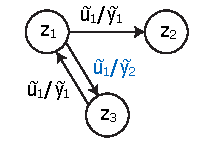
\includegraphics[width=0.6\columnwidth]{figures/fsm_nondeterministic.pdf}
\end{figure}


\subsection{Events}
\subsubsection{Input/Output events}
\textbf{Input events:} ~\\
The $j$-th event of the $i$-th input signal is defined as:
$$
	IE^{(i)}_j
$$

\textbf{Output events:} ~\\
The $j$-th event of the $i$-th output signal is defined as:
$$
	OE^{(i)}_j
$$

\subsubsection{Multiple Signals}
\textbf{Input alphabet:} ~\\
The input symbols based on the input signals are defined as $(i_1 \not = i_2 \not = \dots)$:
$$
	\begin{array}{c}
		\tilde u_1 \hat = \{IE_{j_1}^{(i)}\} \\
		\tilde u_2 \hat = \{IE_{j_2}^{(i)}\} \\
		\vdots \\
		\tilde u_m \hat = \{IE_{j_1}^{(l)}\} \\
		\vdots \\
		\tilde u_n \hat = \{IE_{j_1}^{(i_1)}, IE_{j_2}^{(i_2)}\} \\
		\vdots \\
		\tilde u_o \hat = \{IE_{j_1}^{(i_1)}, IE_{j_2}^{(i_2)}, IE_{j_3}^{(i_3)}\} \\
		\vdots \\
		\vdots \\
	\end{array}
$$

\textbf{Output alphabet:} ~\\
The output symbols based on the output signals are defined as $(i_1 \not = i_2 \not = \dots)$:
$$
	\begin{array}{c}
		\tilde y_1 \hat = \{OE_{j_1}^{(i)}\} \\
		\tilde y_2 \hat = \{OE_{j_2}^{(i)}\} \\
		\vdots \\
		\tilde y_m \hat = \{OE_{j_1}^{(k)}\} \\
		\vdots \\
		\tilde y_n \hat = \{OE_{j_1}^{(i_1)}, OE_{j_2}^{(i_2)}\} \\
		\vdots \\
		\tilde y_o \hat = \{OE_{j_1}^{(i_1)}, OE_{j_2}^{(i_2)}, OE_{j_3}^{(i_3)}\} \\
		\vdots \\
		\vdots \\
	\end{array}
$$

\subsubsection{Don't care-Event}
Any event is allowed for the $i$-th signal \\
\textbf{Input:}
$$
	\{IE^{(i)}_*\} ≡ \{\} \lor \{IE^{(i)}_1\} \lor \{IE^{(i)}_2\} \lor \dots
$$

\textbf{Output:}
$$
	\{OE^{(i)}_*\} ≡ \{\} \lor \{OE^{(i)}_1\} \lor \{OE^{(i)}_2\} \lor \dots
$$

\subsection{Input/Output Sequences}
\textbf{Input sequence:} \\
$$
	\bar u = (u(t_0), u(t_1), \dots), \tab \forall k : u(t_k) \in \mathcal U
$$

\textbf{Output sequence:} \\
$$
	\bar y = (y(t_0), y(t_1), \dots), \tab \forall k : y(t_k) \in \mathcal Y
$$

\textbf{Input-Output Sequence}
$$
	IOS = (\bar u, \bar y)
$$

\textbf{Set of Input-Output Sequences} \\
Set of all possible input-output sequences
$$
	SIOS = \{(\bar u, \bar y) | \bar y \text{ is an output sequence of the input sequence } \bar u = (u(t_0), u(t_1), \dots), \forall k : u(t_k) \in \mathcal U\}
$$

\subsection{Abstraction}
\subsubsection{Definition}
An FSA $A_B$ is an abstraction of an FSA $A_A$, if
$$
	SIOS_A \subseteq SIOS_B
$$

\subsubsection{Properties}
\begin{itemize}
	\item \textbf{Number of states:} Abstracted FSA has fewer states than the original FSA → Easier to analyze
	\item \textbf{Liveness:} If all input-output sequences in $SIOS_B$ fulfill a property, then all sequences in $SIOS_A$ fulfill this property
	\item \textbf{Safety:} If no input-output sequence of $SIOS_B$ fulfills a property, then no input-output sequence of $SIOS_A$ fulfills this property
\end{itemize}

\subsection{Simulation}
\subsubsection{Definition}
An FSA $A_B$ simulates an FSA $A_A$, if there exists a simulation relation $\mathcal S_{AB}$, so that
\begin{itemize}
	\item the initial states are in the simulation relation:
	$$
		(z_A(0), z_B(0)) \in \mathcal S_{AB}
	$$
	\item for each transition, there exists a transition in the other FSA, so that the new states are within the simulation relation:
	$$
		\forall u(k) \in \mathcal U, \forall(z_A(k + 1), y_A(k)) \in h_A(z_A(k), u(k))
	$$
	$$
		\exists (z_B(k + 1), y_B(k)) \in h_B(z_B(k), u(k)):
	$$
	$$
		(z_A(k), z_B(k)) \in S_{AB} \land (z_A(k + 1), z_B(k + 1)) \in S_{AB} \land y_A(k) = y_B(k)
	$$
\end{itemize}

\subsubsection{Verification}
$\mathcal S_{AB} = \{(z_{A,i1}, z_{B, i1}), (z_{A,i2}, z_{B, i2}), \dots \}, \tab z_{A, i1}, z_{A, i2}, \dots \in \mathcal Z_A, z_{B, i1}, z_{B, i2}, \dots \in \mathcal Z_B$ \\
 
\begin{tabular}{c|c|c}
	&& $(z_A(k), z_B(k)) \in S_{AB}$ \\
	&& $\land (z_A(k + 1), z_B(k + 1)) \in S_{AB} $ \\
	transition & simulating transition & $\land y_A(k) = y_B(k)$ \\
	\hline
	$(z_A(k), u(k)) → (z_A(k + 1), y_A(k))$ & $(z_B(k), u(k)) → (z_B(k + 1), y_B(k))$ & \\
	$\vdots$ & $\vdots$ & $\vdots$ 
\end{tabular}

\subsubsection{Properties}
\begin{itemize}
	\item \textbf{Abstraction:} An FSA that simulates another FSA is also an abstraction of that FSA
	\item \textbf{Bisimulation:} An FSA $A_B$ simulates an FSA $A_A$ and vice versa.
\end{itemize}


\section{Petri Nets}
\subsection{Definition}
$$
	PN = (\mathcal P, \mathcal T, \mathcal A)
$$ where
$$
	\begin{array}{ll}
		\mathcal P = \{P_1, \dots, P_{n_p}\} & \text{set of places} \\
		\mathcal T = \{T_1, \dots, T_{n_T}\} & \text{set of transitions} \\
		\mathcal A \subseteq \mathcal P \times \mathcal T \cup \mathcal T \times \mathcal P & \text{set of arcs} \\
		\mathcal P \cap \mathcal T = \emptyset
	\end{array}
$$

\textbf{Pre- and post-arcs:} \\
$$
	\begin{array}{ll}
		\mathcal{PRE} \subseteq \mathcal P \times \mathcal T & \text{Set of pre-arcs} \\
		\mathcal{POST} \subseteq \mathcal T \times \mathcal P & \text{Set of post-arcs}
	\end{array}
$$

\textbf{Pre- and post-places:} \\
$$
	\begin{array}{ll}
		\bullet T_i = \{p \in \mathcal P | (p, T_i) \in \mathcal A\} & \text{Pre-places of } T_i \\
		T_i \bullet = \{p \in \mathcal P | (T_i, p) \in \mathcal A\} & \text{Post-places of } T_i
	\end{array}
$$

\textbf{Pre- and post-transitions:} \\
$$
	\begin{array}{ll}
		\bullet P_i = \{t \in \mathcal T | (t, P_i) \in \mathcal A\} & \text{Pre-transitions of } P_i \\
		P_i \bullet = \{t \in \mathcal T | (P_i, t) \in \mathcal A\} & \text{Post-transitions of } P_i
	\end{array}
$$

\subsection{Graphical Representation}
\begin{figure}[H]
	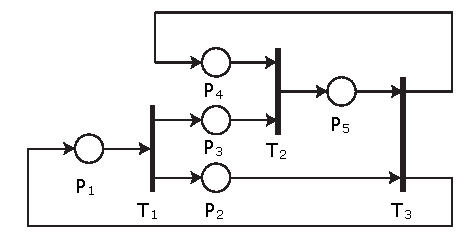
\includegraphics[width=0.7\columnwidth]{figures/petri_net.pdf}
\end{figure}

\subsection{Place/Transition Petri Nets}









\pagebreak
\section*{Notes}
This is a summary of the lecture~\lecture~of the Technical University Munich.
This lecture was presented by~\lecturer~in the~\semseter.
This summary was created by Gaida B.
All provided information is without guarantee.


%\section*{References}
%author. \textit{title}. publisher. location, year, 

\end{document}

%TODO check for todos








